\documentclass[10pt]{article}
\usepackage[english]{babel}
\usepackage{../../../../lib/tex/naproche}
\usepackage{amssymb}
\usepackage{mathtools} % for \coloneq

\usepackage{stex-highlighting}
\providebool{emph} % "\newbool{emph}" does not work...
\setbool{emph}{false}
\colorlet{emphcolor}{violet}
\let\oldemph\emph
\renewcommand\emph[1]{\setbool{emph}{true}\ifbool{forthel}{\textcolor{emphcolor}{\itshape#1}}{\oldemph{#1}}\setbool{emph}{false}}
\renewcommand{\varemph}[1]{\ifbool{emph}{\textcolor{emphcolor}{#1}}{\textcolor{black}{#1}}}

\usepackage[right=6cm,left=3cm,bottom=3cm,marginparwidth=5cm]{geometry}

\usepackage{fancyhdr}
\renewcommand{\sectionmark}[1]{\markboth{#1}{}} 
\def\libarchive{}
\pagestyle{fancy}
\fancyhead[L]{\libarchive}
\fancyhead[C]{\nouppercase\leftmark}  % section title
\fancyhead[R]{\thepage}               % page number
\fancyfoot[C]{}                       % No page number in footer

\usepackage[nobottomtitles]{titlesec}
\titlespacing*{\section}{0pt}{30pt}{0pt}
\titlespacing*{\subsection}{0pt}{30pt}{0pt}
\titlespacing*{\subsubsection}{0pt}{30pt}{0pt}

\documentclass[12pt,oneside]{book}

\usepackage[foundations]{../../lib/tex/naproche}
\usepackage{../../lib/tex/libraries}
\usepackage{graphicx}
\usepackage{float}
\usepackage{caption}
\usepackage{footnote}

\makesavenoteenv{tabular} % Make footnotes work in tabular environments


\title{Foundations of Mathematics}
\author{Marcel Schütz}
\date{2022}

\begin{document}
  \maketitle

  \tableofcontents

  \begin{figure}[H]
    \centering
    \fbox{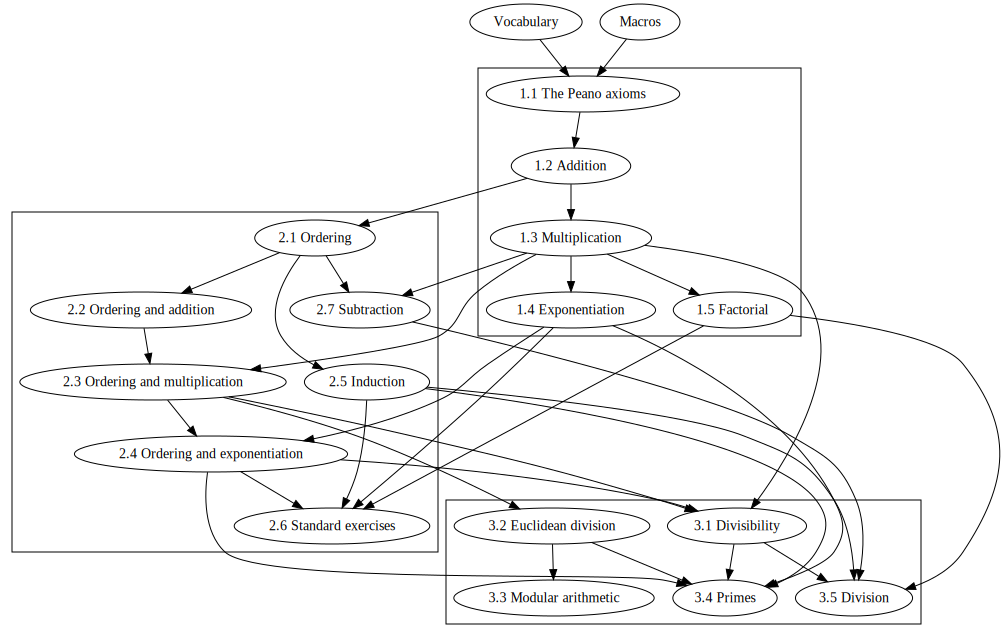
\includegraphics[width=0.9\linewidth]{./dependency-graph/graph.png}}
    \caption*{Interdependencies of the chapters}
  \end{figure}


  \section*{Introduction}

  This is a library providing a foundation of mathematics based on a
  Kelley-Morse like class theory with urelements.
  It introduces common operations on classes like unions or intersections
  (\cref{chapter:classes}) together with detailed proofs of their algebraic
  properties (\cref{chapter:computation-laws-for-classes}), the symmetric
  difference of two classes (\cref{chapter:symmetric-difference}) and the
  notions of ordered pairs and Cartesian products
  (\cref{chapter:pairs-and-products}) as well as proofs of the algebraic
  properties of the latter (\cref{chapter:computation-laws-for-products}).
  Moreover, it provides common operations on maps (\cref{chapter:maps}), various
  properties of images and preimages (\cref{chapter:image-and-preimage}) and the
  notions of injectivity, surjectivity, bijectivity
  (\cref{chapter:injections-surjections-bijections}) and invertibility of maps
  (\cref{chapter:invertible-maps}).
  The library provides an axiom system characterizing sets (\cref{chapter:sets})
  and, furthermore, it covers the notions of binary relations
  (\cref{chapter:binary-relations}), fixed-points of subset preserving maps
  (\cref{chapter:fixed-points}), including and equinumerosity
  (\cref{chapter:equinumerosity}).

  As two famous results it includes the Knaster-Tarski fixed point theorem
  (\cref{FOUNDATIONS_12_8420450166112256}) and the Cantor-Schröder-Bernstein
  theorem (\cref{FOUNDATIONS_13_1913663275401216}).

  \paragraph*{Usage.}
  At the very beginning of each chapter you can find the name of its source
  file, e.g. \path{foundations/sections/01_classes.ftl.tex} for
  \cref{chapter:classes}. This filename can be used to import the chapter via
  \Naproche's \texttt{readtex} instruction to another ForTheL text, e.g.:
  \begin{center}
    \verb`[readtex \path{foundations/sections/01_classes.ftl.tex}]`
  \end{center}

  \paragraph*{Checking times.}
  The checking times for each of the chapters may vary from computer to
  computer, but on mid-range hardware they are likely to be similar to those
  given in table below:

  \begin{center}
    \begin{tabular}{c|c|c}

      & \multicolumn{2}{c}{\textbf{Checking time}}
      \\
      \textbf{Chapter}
      & \textbf{without dependencies}     & \textbf{with dependencies}
      \\ \hline
      \ref{chapter:classes}
      & 00:04 min                         & 00:04 min
      \\
      \ref{chapter:computation-laws-for-classes}
      & 00:12 min                         & 00:16 min
      \\
      \ref{chapter:symmetric-difference}
      & 00:32 min                         & 00:48 min
      \\
      \ref{chapter:pairs-and-products}
      & 00:08 min                         & 00:12 min
      \\
      \ref{chapter:computation-laws-for-products}
      & 01:36 min                         & 01:56 min
      \\
      \ref{chapter:maps}
      & 01:13 min                         & 01:25 min
      \\
      \ref{chapter:image-and-preimage}
      & 01:28 min                         & 02:53 min
      \\
      \ref{chapter:injections-surjections-bijections}
      & 00:38 min                         & 02:03 min
      \\
      \ref{chapter:invertible-maps}
      & 02:20 min                         & 04:23 min
      \\
      \ref{chapter:sets}
      & 02:17 min                         & 06:40 min
      \\
      \ref{chapter:binary-relations}
      & 00:14 min                         & 06:54 min
      \\
      \ref{chapter:fixed-points}
      & 00:33 min                         & 07:13 min
      \\
      \ref{chapter:equinumerosity}
      & 01:48 min                         & 09:01 min
    \end{tabular}
  \end{center}


  \subfile{sections/01_classes.ftl.tex}
  \subfile{sections/02_computation-laws-for-classes.ftl.tex}
  \subfile{sections/03_symmetric-difference.ftl.tex}
  \subfile{sections/04_pairs-and-products.ftl.tex}
  \subfile{sections/05_computation-laws-for-products.ftl.tex}
  \subfile{sections/06_maps.ftl.tex}
  \subfile{sections/07_image-and-preimage.ftl.tex}
  \subfile{sections/08_injections-surjections-bijections.ftl.tex}
  \subfile{sections/09_invertible-maps.ftl.tex}
  \subfile{sections/10_sets.ftl.tex}
  \subfile{sections/11_binary-relations.ftl.tex}
  \subfile{sections/12_fixed-points.ftl.tex}
  \subfile{sections/13_equinumerosity.ftl.tex}
\end{document}

\usepackage{amssymb}

\newcommand{\Nat}{\mathbb{N}}
\newcommand{\Prime}{\mathbb{P}}
\renewcommand{\succ}{\textrm{succ}}
\newcommand{\pred}{\textrm{pred}}
\newcommand{\add}{\textrm{add}}
\newcommand{\mul}{\textrm{mul}}
\renewcommand{\exp}{\textrm{exp}}
\newcommand{\fac}{\textrm{fac}}
\renewcommand{\div}{\mathop{\textrm{div}}}
\renewcommand{\mod}{\mathop{\textrm{mod}}}

\begin{document}
  \begin{imports}
    \begin{forthel}
      %[prove off][check off]
      [readtex \path{libraries/source/arithmetics/divisibility.ftl.tex}]
      [readtex \path{libraries/source/arithmetics/subtraction.ftl.tex}]
      %[prove on][check on]
    \end{forthel}
  \end{imports}


  \section*{Even and Odd Numbers}

  \subsection*{Definition}

  \begin{forthel}
    \begin{definition}\printlabel{ARITHMETIC_15_4521358965847512}
      Let $n$ be a natural number.
      $n$ is even iff $n$ is divisible by $2$.
    \end{definition}
  \end{forthel}

  \begin{forthel}
    \begin{definition}\printlabel{ARITHMETIC_15_1023652125874596}
      Let $n$ be a natural number.
      $n$ is odd iff $n$ is not divisible by $2$.
    \end{definition}
  \end{forthel}

  \begin{forthel}
    \begin{proposition}\printlabel{ARITHMETIC_15_0236985458752156}
      Let $n$ be a natural number.
      $n$ is even iff $n = 2 \cdot m$ for some natural number $m$.
    \end{proposition}
    \begin{proof}
      Case $n$ is even.
        Then $2$ divides $n$.
        Hence $n = 2 \cdot m$ for some natural number $m$.
      End.

      Case $n = 2 \cdot m$ for some natural number $m$.
        Then $2$ divides $n$.
        Hence $2$ is even.
      End.
    \end{proof}
  \end{forthel}

  \begin{forthel}
    \begin{proposition}\printlabel{ARITHMETIC_15_1023512547854265}
      Let $n$ be a natural number.
      $n$ is odd iff $n = (2 \cdot m) + 1$ for some natural number $m$.
    \end{proposition}
    \begin{proof}
      Case $n$ is odd.
        (a) Define $\Phi = \{ n' \in \Nat \mid$ if $n'$ is odd then $n' = (2 \cdot m) + 1$ for some natural number $m \}$.

        (1) $\Phi$ contains $0$.
        Indeed $0$ is not odd.

        (2) For all $n' \in \Phi$ we have $n' + 1 \in \Phi$. \\
        Proof.
          Let $n' \in \Phi$.

          Let us show that if $n' + 1$ is odd then $(n' + 1) = (2 \cdot m) + 1$ for some natural number $m$.
            Assume that $n' + 1$ is odd.

            Case $n'$ is even.
              Take a natural number $m$ such that $n' = 2 \cdot m$.
              Then $n' + 1 = (2 \cdot m) + 1$.
            End.

            Case $n'$ is odd.
              Take a natural number $m$ such that $n' = (2 \cdot m) + 1$.
              Then $n' + 1
                = ((2 \cdot m) + 1) + 1
                = (2 \cdot m) + (1 + 1)
                = (2 \cdot m) + 2
                = 2 \cdot (m + 1)$.
              Hence $2$ divides $n'$.
              Thus $n'$ is even.
              Contradiction.
            End.
          End.
        Qed.

        Then $\Phi$ contains every natural number (by \printref{ARITHMETIC_01_4764664342773760}).
        Hence $n$ is odd iff $n = (2 \cdot m) + 1$ for some natural number $m$ (by a).
      End.

      Case $n = (2 \cdot m) + 1$ for some natural number $m$.
        Consider a natural number $m$ such that $n = (2 \cdot m) + 1$.
        Assume that $n$ is even.
        Then we can take a natural number $k$ such that $n = 2 \cdot k$.
        Then we have $2 \cdot k = (2 \cdot m) + 1$.
        Hence $2$ divides $(2 \cdot m) + 1$.
        Thus $2$ divides $1$.
        Indeed $2$ divides $2 \cdot m$.
        Contradiction.
      End.
    \end{proof}
  \end{forthel}

  \begin{forthel}
    \begin{proposition}\printlabel{ARITHMETIC_15_1023652154254789}
      Let $n$ be a natural number.
      $n$ is odd iff $n = (2 \cdot m) - 1$ for some positive natural number $m$.
    \end{proposition}
    \begin{proof}
      Case $n$ is odd.
        Consider a natural number $k$ such that $n = (2 \cdot k) + 1$.
        Take $m = k + 1$.
        Then $n
          = (2 \cdot k) + 1
          = (2 \cdot (k + 0)) + 1
          = (2 \cdot (k + (1 - 1))) + 1
          = (2 \cdot ((k + 1) - 1)) + 1
          = (2 \cdot (m - 1)) + 1
          = ((2 \cdot m) - (2 \cdot 1)) + 1
          = ((2 \cdot m) - 2) + 1
          = (2 \cdot m) - 1$.
      End.

      Case $n = (2 \cdot m) - 1$ for some positive natural number $m$.
        Consider a positive natural number $m$ such that $n = (2 \cdot m) - 1$.
        Take $k = m - 1$.
        Then $n
          = (2 \cdot m) - 1
          = (2 \cdot (m + 0)) - 1
          = (2 \cdot (m + (1 - 1))) - 1
          = (2 \cdot ((m + 1) - 1)) - 1
          = (2 \cdot ((m - 1) + 1)) - 1
          = (2 \cdot (k + 1)) - 1
          = ((2 \cdot k) + (2 \cdot 1)) - 1
          = ((2 \cdot k) + 2) - 1
          = (2 \cdot k) + (2 - 1)
          = (2 \cdot k) + 1$.
        Hence $n$ is odd.
      End.
    \end{proof}
  \end{forthel}


  \subsection*{Addition of Even and Odd Numbers}

  \begin{forthel}
    \begin{proposition}\printlabel{ARITHMETIC_15_7845441256365256}
      Let $n, m$ be natural numbers.
      Assume that $n$ and $m$ are even.
      Then $n + m$ is even.
    \end{proposition}
    \begin{proof}
      Take natural numbers $k, l$ such that $n = 2 \cdot k$ and $m = 2 \cdot l$.
      Then $n + m
        = (2 \cdot k) + (2 \cdot l)
        = 2 \cdot (k + l)$.
      Hence $n + m$ is even.
    \end{proof}
  \end{forthel}

  \begin{forthel}
    \begin{proposition}\printlabel{ARITHMETIC_15_1023655256985478}
      Let $n, m$ be natural numbers.
      Assume that $n$ is even and $m$ is odd.
      Then $n + m$ is odd.
    \end{proposition}
    \begin{proof}
      Take natural numbers $k, l$ such that $n = 2 \cdot k$ and $m = (2 \cdot l) + 1$.
      Then $n + m
        = (2 \cdot k) + ((2 \cdot l) + 1)
        = ((2 \cdot k) + (2 \cdot l)) + 1
        = (2 \cdot (k + l)) + 1$.
      Hence $n + m$ is odd.
    \end{proof}
  \end{forthel}

  \begin{forthel}
    \begin{corollary}\printlabel{ARITHMETIC_15_0125412589658745}
      Let $n, m$ be natural numbers.
      Assume that $n$ is odd and $m$ is even.
      Then $n + m$ is odd.
    \end{corollary}
  \end{forthel}

  \begin{forthel}
    \begin{proposition}\printlabel{ARITHMETIC_15_1023659854785412}
      Let $n, m$ be natural numbers.
      Assume that $n$ and $m$ are odd.
      Then $n + m$ is even.
    \end{proposition}
    \begin{proof}
      Take natural numbers $k, l$ such that $n = (2 \cdot k) + 1$ and $m = (2 \cdot l) + 1$.
      Then $n + m
        = ((2 \cdot k) + 1) + ((2 \cdot l) + 1)
        = (((2 \cdot k) + 1) + (2 \cdot l)) + 1
        = ((2 \cdot k) + (1 + (2 \cdot l))) + 1
        = ((2 \cdot k) + ((2 \cdot l) + 1)) + 1
        = (((2 \cdot k) + (2 \cdot l)) + 1) + 1
        = ((2 \cdot k) + (2 \cdot l)) + (1 + 1)
        = ((2 \cdot k) + (2 \cdot l)) + 2
        = (2 \cdot (k + l)) + 2
        = 2 \cdot ((k + l) + 1)$.
        Hence $n + m$ is even.
    \end{proof}
  \end{forthel}


  \subsection{Subtraction of even and odd numbers}

  \begin{forthel}
    \begin{proposition}\printlabel{ARITHMETIC_15_8748569852145203}
      Let $n, m$ be natural numbers such that $n \geq m$.
      Assume that $n, m$ are even.
      Then $n - m$ is even.
    \end{proposition}
    \begin{proof}
      Take natural numbers $k, l$ such that $n = 2 \cdot k$ and $m = 2 \cdot l$.
      Then $k \geq l$.
      Hence $n - m
        = (2 \cdot k) - (2 \cdot l)
        = 2 \cdot (k - l)$.
      Thus $n - m$ is even.
    \end{proof}
  \end{forthel}

  \begin{forthel}
    \begin{proposition}\printlabel{ARITHMETIC_15_0125412036589958}
      Let $n, m$ be natural numbers such that $n \geq m$.
      Assume that $n$ is even and $m$ is odd.
      Then $n - m$ is odd.
    \end{proposition}
    \begin{proof}
      Take natural numbers $k, l$ such that $n = 2 \cdot k$ and $m = (2 \cdot l) + 1$.
      Then $k \geq l$ and $2 \cdot (k - l) \geq 1$.
      Hence $n - m
        = (2 \cdot k) - ((2 \cdot l) + 1)
        = ((2 \cdot k) - (2 \cdot l)) - 1
        = (2 \cdot (k - l)) - 1$.
      Thus $n - m$ is odd.
    \end{proof}
  \end{forthel}

  \begin{forthel}
    \begin{corollary}\printlabel{ARITHMETIC_15_1021458745896523}
      Let $n, m$ be natural numbers such that $n \geq m$.
      Assume that $n$ is odd and $m$ is even.
      Then $n - m$ is odd.
    \end{corollary}
    \begin{proof}
      Take natural numbers $k, l$ such that $n = (2 \cdot k) + 1$ and $m = 2 \cdot l$.
      Then $k \geq l$.
      Hence $n - m
        = ((2 \cdot k) + 1) - (2 \cdot l)
        = (1 + (2 \cdot k)) - (2 \cdot l)
        = 1 + ((2 \cdot k) - (2 \cdot l))
        = ((2 \cdot k) - (2 \cdot l)) + 1
        = (2 \cdot (k - l)) + 1$.
      Indeed $((2 \cdot k) - (2 \cdot l)) = 2 \cdot (k - l)$. %!
      Thus $n - m$ is odd.
    \end{proof}
  \end{forthel}

  \begin{forthel}
    \begin{proposition}\printlabel{ARITHMETIC_15_0125478854587412}
      Let $n, m$ be natural numbers such that $n \geq m$.
      Assume that $n, m$ are odd.
      Then $n - m$ is even.
    \end{proposition}
    \begin{proof}
      Take natural numbers $k, l$ such that $n = (2 \cdot k) + 1$ and $m = (2 \cdot l) + 1$.
      Then $k \geq l$.
      Indeed $2 \cdot k \geq 2 \cdot l$.
      Hence $1 + (2 \cdot k) \geq 2 \cdot l$.
      Thus $n - m
        = ((2 \cdot k) + 1) - ((2 \cdot l) + 1)
        = ((1 + (2 \cdot k)) - (2 \cdot l)) - 1
        = (1 + ((2 \cdot k) - (2 \cdot l))) - 1
        = (1 + (2 \cdot (k - l))) - 1
        = ((2 \cdot (k - l)) + 1) - 1
        = 2 \cdot (k - l)$.
      Indeed $((2 \cdot k) - (2 \cdot l)) = 2 \cdot (k - l)$. %!
      Therefore $n - m$ is even.
    \end{proof}
  \end{forthel}


  \subsection*{Multiplication of Even and Odd Numbers}

  \begin{forthel}
    \begin{proposition}\printlabel{ARITHMETIC_15_0125698547589652}
      Let $n, m$ be natural numbers.
      Assume that $n$ is even or $n$ is even.
      Then $n \cdot m$ is even.
    \end{proposition}
    \begin{proof}
      Case $n$ is even.
        Take a natural number $k$ such that $n = 2 \cdot k$.
        Then $n \cdot m
          = (2 \cdot k) \cdot m
          = 2 \cdot (k \cdot m)$.
        Hence $n \cdot m$ is even.
      End.

      Case $m$ is even.
        Take a natural number $l$ such that $m = 2 \cdot l$.
        Then $n \cdot m
          = n \cdot (2 \cdot l)
          = (n \cdot 2) \cdot l
          = (2 \cdot n) \cdot l
          = 2 \cdot (n \cdot l)$.
        Hence $n \cdot m$ is even.
      End.
    \end{proof}
  \end{forthel}

  \begin{forthel}
    \begin{proposition}\printlabel{ARITHMETIC_15_0236596587452145}
      Let $n, m$ be natural numbers.
      Assume that $n$ and $m$ are odd.
      Then $n \cdot m$ is odd.
    \end{proposition}
    \begin{proof}
      Take natural numbers $k, l$ such that $n = (2 \cdot k) + 1$ and $m = (2 \cdot l) + 1$.
      Then $n \cdot m
        = ((2 \cdot k) + 1) \cdot m
        = ((2 \cdot k) \cdot m) + (1 \cdot m)
        = ((2 \cdot k) \cdot m) + m
        = (2 \cdot (k \cdot m)) + m$.
      $2 \cdot (k \cdot m)$ is even and $m$ is odd.
      Hence $(2 \cdot (k \cdot m)) + m$ is odd.
      Therefore $n \cdot m$ is odd.
    \end{proof}
  \end{forthel}
\end{document}